\documentclass{article}

\usepackage{iclr2026_conference,times}
\input{math_commands.tex}
\usepackage{graphicx}
\usepackage{booktabs}
\usepackage{amsmath}
\usepackage{amssymb}
\usepackage{amsthm}
\usepackage{url}

\newtheorem{theorem}{Theorem}
\newtheorem{proposition}{Proposition}
\newtheorem{definition}{Definition}

\title{Active Constraint Signatures: Discovering Binding Constraint Families Before Robot Planning}

\author{Anonymous Authors}

\begin{document}

\maketitle

\begin{center}
{\small Submission-hardening version: v2 (2026-06-12).}
\end{center}

\begin{abstract}
Robot planners often encounter constraints only after search has already begun: a geometric stream fails, a feasibility classifier rejects an edge, or execution exposes that a planned manipulation is invalid. This paper argues that for many embodied planning problems the active constraint family is an instance-level property that should be discovered before planning. We introduce Active Constraint Signatures (ACS), a pre-planning certificate that maps scene cues and cheap diagnostic probes to the set of physical constraint families currently binding, then masks entire action families before graph or task-and-motion search. ACS is not a new verifier or repair module; it changes the object passed to the planner from a per-edge feasibility oracle to an active-family certificate. We give a finite-graph condition under which a sound signature preserves completeness for the pruned problem and derive when ACS is cheaper than edge verification or repair. A reproducible robot-task abstraction with eight physical constraint families shows the intended regime: at active-family probability 0.35, ACS has median total cost 22.01 versus 261.01 for blind repair, 65.16 for family-level repair, and 116.79 for a perfect edge verifier. The evidence is intentionally scoped: ACS assumes a known constraint vocabulary and is not yet a physical-robot result.
A v2 signature-noise stress narrows the claim: at active-family probability
0.35, the valid-plan rate falls from 1.000 with exact signatures to 0.887 when
5\% of active families are missed, 0.766 when 10\% are missed, and 0.584 when
20\% are missed. ACS is therefore a planner-facing representation for reliable
family diagnostics, not a solution to noisy constraint discovery.
\end{abstract}

\section{Introduction}

Robot planning is full of constraints, but the timing of constraint discovery is often treated as incidental. A task-and-motion planner may optimistically branch over symbolic actions and call geometric streams later \citep{garrett2020pddlstream,vu2024coast}; a logic-geometric planner may discover infeasibility through constrained optimization \citep{toussaint2015logic,ly2024rlgp}; a learned feasibility model may reject candidate actions during search \citep{xu2022accelerating,aitbouhsain2023simultaneous}; and a repair system may modify a plan after a symbolic-geometric failure. These mechanisms are powerful, but they share a hidden assumption: discovering which constraint families are binding is cheap enough to do inside the ordinary planning loop.

This assumption is false in many embodied settings. A wet floor invalidates many low-friction navigation shortcuts; a fragile payload invalidates a family of fast carry motions; a human exclusion zone invalidates every path through an occupied region; a sealed container invalidates direct pick actions until a tool or opening action is used. In such cases, the first invalid plan is not an isolated mistake. It is evidence that a whole family of tempting actions should never have entered the search frontier.

We study the following mechanism: before planning, infer a compact \emph{active constraint signature} for the current instance. The signature lists modeled physical constraint families that are active, together with the diagnostic source that supports them. The planner then masks action families whose labels intersect that signature. This is a small conceptual shift, but it changes the unit of amortization: one diagnostic probe can remove many invalid edges.

The contribution is deliberately narrow.
\begin{itemize}
    \item We define ACS as an instance-level active-family certificate for robot planning.
    \item We prove that, under exact discovery for the modeled families, masking preserves completeness with respect to the pruned feasible graph.
    \item We derive a simple cost condition separating ACS from edge-by-edge verification and repair-after-planning.
    \item We provide a runnable simulator that compares ACS to blind repair, failure-generalizing repair, a perfect edge verifier, and an oracle signature.
\end{itemize}

The result is not a claim that ACS discovers arbitrary new physics, replaces motion planning, or has been validated on hardware. Rather, it is a pressure test for the field assumption that constraints can be discovered late without changing the planning problem.

\section{Related Work and Novelty Boundary}

\paragraph{Task and motion planning.}
Classic task-and-motion planning integrates symbolic search with geometric reasoning \citep{wolfe2010combined,kaelbling2011hierarchical,lagriffoul2014efficiently}. Later systems made this integration incremental, factored, stream-based, or optimization-based \citep{dantam2016incremental,dantam2018incremental,garrett2017ffrob,garrett2018sampling,garrett2020pddlstream,toussaint2015logic}. Recent work adds reachability guidance, stream constraints, temporal specifications, and long-horizon construction or manipulation structure \citep{takano2021continuous,hartmann2022long,ly2024rlgp,vu2024coast}. ACS does not dispute this line: it assumes a downstream planner and asks whether the active constraint family should be inferred before that planner expands its search space.

\paragraph{Learning constraints and feasibility.}
Learning has been used to induce skill models, geometric constraints, action abstractions, and feasibility checks for planning \citep{wang2021compositional,curtis2022discovering,ren2022learning,xu2022accelerating,aitbouhsain2023simultaneous}. These methods make ``learning constraints'' too broad to be a novel claim. The boundary here is more specific: ACS produces one active-family signature per instance, not a score or rejection for each candidate edge.

\paragraph{Language-guided and specification-guided planning.}
Recent work translates task constraints from language or uses large vision-language models to guide long-horizon planning \citep{chen2024autotamp,guo2025castl,yang2025guiding}. ACS is complementary: the active signature may be produced by language, perception, or robot probes, but its planner-facing role is to certify which constraint families are binding before search.

\section{Problem Setting}

Let $G=(V,E)$ be a finite directed planning graph for a robot task abstraction. An edge $e \in E$ is a macro-action, stream call, or skill invocation. Let $\mathcal{C}=\{c_1,\dots,c_K\}$ be a known vocabulary of physical constraint families. Each edge has a label set $\ell(e)\subseteq\mathcal{C}$ containing the families that would invalidate that edge if active. A problem instance has an unknown active set $A\subseteq\mathcal{C}$. Edge $e$ is valid iff $\ell(e)\cap A=\emptyset$.

This abstraction intentionally covers only constraints that can be grouped into reusable families. It is suitable for constraints such as fragile payloads, narrow passages, human exclusion regions, terrain restrictions, payload limits, tool requirements, or perception-mode restrictions. It is not an open-world model of all possible physical invalidity.

\begin{definition}[Active Constraint Signature]
An Active Constraint Signature for an instance is a set $\hat{A}\subseteq\mathcal{C}$ returned before planning by a diagnostic procedure $D$. The planner searches the masked graph
\[
G_{\hat{A}} = (V,\{e\in E:\ell(e)\cap \hat{A}=\emptyset\}).
\]
\end{definition}

In the ideal case, $D$ uses scene observations and bounded robot probes to return $\hat{A}=A$. In practice, $D$ could be a classifier, a ruleset, a set of physical tests, or a hybrid. This paper studies the planner-side consequences of making $\hat{A}$ explicit.

\section{Method: Planning With Active Constraint Signatures}

ACS has three steps.
\begin{enumerate}
    \item \textbf{Diagnose.} Query scene cues and cheap probes for every modeled constraint family, producing evidence such as ``payload is fragile'', ``route crosses wet floor'', or ``container is sealed''.
    \item \textbf{Certify.} Convert evidence into a signature $\hat{A}$ and attach the family-level mask it induces.
    \item \textbf{Plan.} Run the downstream planner on $G_{\hat{A}}$, so that entire action families are removed before expansion.
\end{enumerate}

This differs from a verifier because the diagnostic is paid per family or per instance, not per candidate edge. It differs from repair because no invalid execution is needed to expose the first member of a family. It differs from ordinary precondition learning because the learned object is not only an operator schema; it is a problem-instance active-set certificate.

\subsection{Formal Guarantee}

\begin{theorem}[Sound-mask completeness]
Assume $G$ is finite, the downstream planner is complete on any subgraph of $G$, and ACS returns the exact modeled active set $\hat{A}=A$. If there exists a path from start to goal using only valid edges, planning on $G_{\hat{A}}$ returns such a path. Every returned path is valid with respect to the modeled active constraints.
\end{theorem}

\begin{proof}
By construction, $G_{\hat{A}}$ contains exactly those edges $e$ for which $\ell(e)\cap\hat{A}=\emptyset$. Since $\hat{A}=A$, this is exactly the set of modeled-valid edges. Any valid path in $G$ is therefore present in $G_{\hat{A}}$, and every path in $G_{\hat{A}}$ is valid. Completeness of the downstream planner on the finite subgraph gives existence of a returned path whenever one exists.
\end{proof}

The theorem is conditional. False negatives can allow invalid edges into search; false positives can remove valid plans. ACS therefore needs abstention, verification, or recovery in noisy deployments. The present paper proves the clean planner-side property and evaluates the cost tradeoff in the exact-signature setting.

\subsection{Cost Condition}

Let $K$ be the number of modeled families, $c_p$ the cost of a diagnostic probe, $M$ the number of candidate edges examined by an edge verifier, and $c_v$ the cost of one verifier call. Ignoring shared downstream search cost, ACS is cheaper than edge verification when
\[
Kc_p < Mc_v.
\]
For repair-after-planning, let $q$ be the number of invalid executions before a successful plan and $c_f$ their cost. ACS beats repair when
\[
Kc_p + \Delta_{\mathrm{search}} < q c_f,
\]
where $\Delta_{\mathrm{search}}$ is the difference in planning computation after masking versus after repair. These inequalities are not universal dominance claims; they identify the regime where active-family discovery changes the economics of planning.

\section{Experiments}

\subsection{Robot-Task Abstraction}

We built a deterministic simulator in which a layered graph represents a robot task plan. Edges are macro-actions such as direct navigation, grasp, carry, inspect, and tool-use choices. Each edge may carry one or two labels from eight physical constraint families: fragile payload, wet floor, narrow passage, human exclusion, thermal contact, payload limit, sealed container, and low-light perception. A task instance samples an active subset. If a family is active, every edge carrying that label is invalid. A conservative safe chain guarantees that a feasible plan exists, but it is more expensive than many tempting invalid branches.

\subsection{Baselines}

We compare five methods.
\begin{itemize}
    \item \textbf{Blind repair}: plan ignoring constraints, execute, blacklist only the failed edge, and replan.
    \item \textbf{Family repair}: after a failed edge, infer the violated family and blacklist that family.
    \item \textbf{Edge verifier}: call a perfect feasibility verifier on every candidate edge considered during Dijkstra search.
    \item \textbf{ACS}: pay one diagnostic probe per family, mask active families, then plan.
    \item \textbf{Oracle signature}: plan with the true active set and no diagnostic cost.
\end{itemize}

Each setting uses 180 random tasks. The cost model is transparent in the released code: expansion cost 0.03, verifier call cost 0.18, probe cost 0.55, invalid execution cost 18.0, and failure cost 250.0. These values are not calibrated to a particular robot; they instantiate the regime where invalid execution and repeated feasibility calls are meaningfully costly.

\begin{figure}[t]
    \centering
    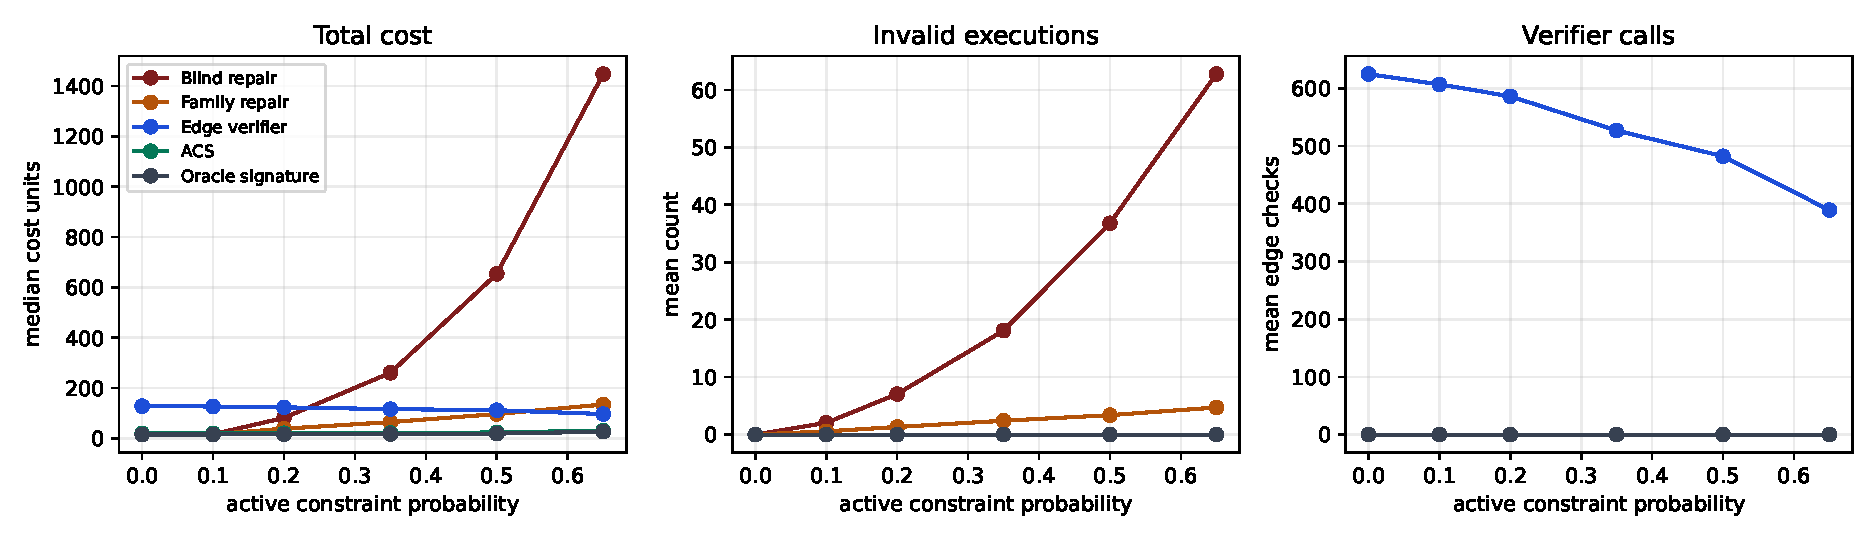
\includegraphics[width=\linewidth]{../figures/main_results.pdf}
    \caption{ACS pays a fixed diagnostic cost and therefore loses when no constraints are active. Once active families create repeated invalid branches, ACS avoids invalid executions and hundreds of verifier calls.}
    \label{fig:main}
\end{figure}

\begin{table}[t]
\centering
\caption{Median total cost. Lower is better.}
\label{tab:cost}
\begin{tabular}{lrrrrr}
\toprule
Active prob. & Blind repair & Family repair & Edge verifier & ACS & Oracle \\
\midrule
0.00 & 15.76 & 15.76 & 128.74 & 20.16 & 15.76 \\
0.20 & 81.93 & 39.07 & 123.76 & 21.05 & 16.65 \\
0.35 & 261.01 & 65.16 & 116.79 & 22.01 & 17.61 \\
0.50 & 653.75 & 97.35 & 112.39 & 24.01 & 19.61 \\
0.65 & 1447.38 & 134.94 & 97.24 & 31.51 & 27.11 \\
\bottomrule
\end{tabular}
\end{table}

\subsection{Results}

Figure~\ref{fig:main} and Table~\ref{tab:cost} show the intended tradeoff. When active probability is 0.00, ACS has no invalid branches to avoid and pays 4.4 extra diagnostic cost relative to blind repair. This is the expected failure mode. At active probability 0.35, ACS has median total cost 22.01, while blind repair reaches 261.01 because it repeatedly discovers one invalid edge at a time. Family repair is much stronger, but still pays for the first failed execution of each discovered family, reaching 65.16. The perfect edge verifier avoids invalid executions but averages 527 verifier calls at active probability 0.35 and has median cost 116.79.

At high active probabilities, blind repair becomes extremely costly because low-cost branches are often invalid. ACS approaches the oracle signature plus a fixed probe overhead. Edge verification improves as many invalid edges are pruned early, but it still pays hundreds of edge checks. These results support the mechanism claim: the value of ACS comes from amortizing family-level discovery before search.

\begin{table}[t]
\centering
\caption{Signature-noise stress at active probability $0.35$. Columns show the
probability that an active family is missed by the diagnostic signature. False
negatives are dangerous because missed active families leave invalid low-cost
branches in the planner.}
\label{tab:signature-noise}
\begin{tabular}{lrrrrr}
\toprule
Metric & 0\% & 2\% & 5\% & 10\% & 20\% \\
\midrule
Valid-plan rate & 1.000 & 0.962 & 0.887 & 0.766 & 0.584 \\
Median total cost & 22.14 & 22.20 & 22.39 & 22.94 & 25.35 \\
Invalid executions & 0.00 & 0.04 & 0.11 & 0.23 & 0.42 \\
\bottomrule
\end{tabular}

\end{table}

Table~\ref{tab:signature-noise} stress-tests the exact-signature assumption. A
2\% active-family miss rate still gives a 0.962 valid-plan rate, but at 5\% the
rate drops to 0.887, at 10\% to 0.766, and at 20\% to 0.584. The median total
cost moves only modestly because failed plans pay the configured failure cost
once, but the validity drop is the important safety signal. The extended CSV
also includes false-positive rows: in this simulator, 5\% and 10\% false
positives preserve a 1.000 valid-plan rate because the conservative untagged
chain remains, though they raise median cost slightly. Less forgiving graphs
could lose completeness under false positives.

\section{Limitations}

The current evidence is a proof-of-mechanism abstraction, not a hardware demonstration. The constraint vocabulary is known. Edge labels are supplied by the simulator. Diagnostics are exact in the main result, and the v2 stress shows that false negatives rapidly undermine plan validity. The cost model is illustrative. A deployed ACS system would need calibrated probes, perception uncertainty, abstention when signatures are ambiguous, recovery from false positives, and integration with continuous motion feasibility checks. The paper should therefore be read as identifying a planning mechanism and evaluation regime, not as closing the full robot-learning problem.

\section{Reproducibility Statement}

The repository contains all source needed to regenerate the evidence: `scripts/run\_experiments.py' runs the simulator, writes raw trials to `results/raw\_trials.csv', aggregates `results/summary.csv', writes the signature-noise stress to `results/signature\_noise\_stress.csv', and produces Figure~\ref{fig:main}. The literature sweep is also scripted: `scripts/literature\_pipeline.py' generates the 1000-paper matrix, 300-paper skim, 225-paper deep-read subset, and 100-paper hostile set. No proprietary data or external robot hardware is required.

\section{Ethics Statement}

ACS is intended to reduce invalid robot actions by identifying active physical constraints before planning. The current paper does not deploy robots around humans. If used in safety-critical settings, false negatives could permit unsafe plans and false positives could block necessary robot behavior. A real system should pair ACS with conservative verification, monitoring, and human-approved safety procedures.

\section{Conclusion}

The paper's central claim is not that robots need constraints; that is already clear from decades of TAMP and motion-planning work. The claim is that, when many candidate actions share latent physical constraint families, the active set should be discovered before planning and represented as a planner-facing signature. ACS gives this idea a name, a formal boundary, and runnable evidence for the regime where it matters.

\bibliography{references}
\bibliographystyle{iclr2026_conference}

\appendix
\section{Corpus Protocol}

Before choosing the thesis, we ran a metadata-driven literature sweep over 24 searches covering robot planning, task-and-motion planning, constraint learning, feasibility prediction, action-model learning, affordances, contact planning, temporal constraints, and plan repair. The script retained 1000 scored entries, designated the top 300 as a serious skim, the top 225 as a deep-read subset, and selected 100 hostile papers most likely to make ACS incremental. The generated artifacts are `docs/related\_work\_matrix.csv', `docs/literature\_map.md', `docs/hostile\_prior\_work.md', and `docs/novelty\_boundary\_map.md'.

\section{Proof Details and Adversarial Cases}

The sound-mask theorem depends on exact signatures. If $\hat{A}\subset A$, a false negative leaves some invalid edges in the graph and downstream verification or execution monitoring is still needed. If $A\subset\hat{A}$, a false positive may remove valid solutions and break completeness. Thus the theorem is best understood as a planner-side decomposition: if diagnostic discovery is sound and complete for the modeled family vocabulary, then the planner inherits the usual complete-search property on the masked graph.

ACS is weakest when constraints are rare, diagnostic probes are expensive, or invalid execution is cheap. It is strongest when a small number of active families invalidate many tempting branches and when verifier calls or failed executions are expensive. These are exactly the conditions expressed by $Kc_p < Mc_v$ and $Kc_p + \Delta_{\mathrm{search}} < q c_f$.

\end{document}
